\documentclass[11pt]{article}

\usepackage[a4paper,margin=1in]{geometry}
\usepackage{amsmath,amssymb,amsthm,mathtools}
\usepackage{booktabs}
\usepackage{graphicx}
\usepackage[colorlinks=true,linkcolor=blue,citecolor=blue,urlcolor=blue]{hyperref}

\graphicspath{{paper/figures/}{figures/}}

\newtheorem{theorem}{Theorem}
\newtheorem{lemma}{Lemma}
\newtheorem{definition}{Definition}
\newtheorem{remark}{Remark}

\DeclareMathOperator*{\argmin}{arg\,min}

\title{Proximal Cyclic Block Coordinate Descent for Euclidean Graph Realization}
\author{}
\date{}

\begin{document}

\maketitle

\begin{abstract}
We consider the problem of realizing a connected weighted graph in \(\mathbb R^K\) by minimizing a quartic least-squares distance objective.  The usual cyclic exact block-coordinate method may fail because the vertex block subproblems can have nonunique minimizers.  We therefore add a proximal term to each block update.  For the anchored formulation with only one fixed vertex, we prove boundedness of the iterates, sufficient decrease, stationarity of accumulation points, and whole-sequence convergence by verifying the standard Kurdyka--\L{}ojasiewicz descent framework.  We also report small reproducible numerical experiments in the planar case \(K=2\), generated by a pure-Python implementation.
\end{abstract}

\section{Introduction}

The \emph{Distance Geometry Problem} (DGP) asks whether a weighted graph can be realized in Euclidean space with prescribed intervertex distances.  Formally, given an integer $K>0$ and a simple undirected graph $G=(V,E)$ with edge weights $d:E\to\mathbb R_+$, one seeks a realization $x:V\to\mathbb R^K$ satisfying
\[
    \|x(i)-x(j)\|=d(\{i,j\}),\qquad \{i,j\}\in E.
\]
We adopt the convention that $x(i)$ denotes the coordinate of vertex $i$.  

The problem was first explicitly formulated by Yemini~\cite{yemini1978} in the context of distributed sensor localization.  Saxe~\cite{saxe1979} later proved that the $K$-embeddability problem is strongly NP-complete for $K=1$ and strongly NP-hard for general $K>1$, establishing the computational difficulty of DGP even in low dimensions.

Applications of DGP span molecular conformation~\cite{more1999}, sensor network localization, and graph drawing, which has renewed algorithmic interest in tractable continuous formulations.  A standard approach replaces the equality constraints by the quartic least-squares objective
\[
    f(x)=\sum_{\{i,j\}\in E}\bigl(\|x_i-x_j\|^2-d_{ij}^2\bigr)^2,
\]
whose global minimizers with $f=0$ are exactly the realizations.  This reformulation converts the combinatorial feasibility question into a (nonconvex, nonsmooth-free) continuous optimization problem accessible to gradient-based methods.

The same quartic loss is central in multidimensional scaling and molecular distance geometry.  Amaral et al.~\cite{amaral2022complexity} developed a high-order regularized coordinate-descent framework for smooth nonconvex box-constrained problems and applied it to such distance-geometry objectives, using low-dimensional point blocks and regularized Taylor models.  Classical convergence results for nonlinear block Gauss--Seidel and BCD methods often require structural assumptions such as uniqueness, pseudoconvexity, or special block geometry, while proximal variants can restore convergence under weaker assumptions~\cite{grippo2000convergence,tseng2001convergence,wright2015coordinate}.  Our aim is more specific: we study exact cyclic vertex updates for the anchored graph-realization objective, add a fixed quadratic proximal term, and isolate the nonunique-minimizer mechanism that can make the unregularized exact method cycle.

For fixed \(K\), a natural coordinate-descent strategy updates one vertex at a time while keeping all others fixed.  This cyclic block-coordinate descent (BCD) scheme is attractive because each block subproblem has only \(K\) variables.  However, exact cyclic BCD may cycle without converging: when a block subproblem has nonunique minimizers, a legal but ``wrong'' choice can create a persistent tie-switching orbit that keeps the objective constant and the iterate step bounded away from zero.

We cure this defect by adding a proximal term to each block update.  The proximal parameter $\mu>0$ penalizes large moves from the current block value and supplies the sufficient-decrease estimate needed for the convergence proof.  The convergence argument follows the now-standard pattern for proximal alternating and descent methods based on sufficient decrease, a relative error estimate, and the Kurdyka--\L{}ojasiewicz (KL) property~\cite{attouch2010proximal,attouch2013convergence,bolte2014proximal}; the graph-specific work is to verify these ingredients for the one-anchor realization objective and the exact cyclic vertex update.

\paragraph{Contributions.}
\begin{enumerate}
    \item We prove boundedness of the one-anchor sublevel sets for connected graphs, which gives compactness without artificial box constraints or additional anchors (Section~\ref{sec:convergence}).
    \item We exhibit a concrete two-cycle for exact cyclic BCD on a planar DGP instance (\(K=2\)) and show analytically that adding a proximal term eliminates the tie-switching mechanism (Section~\ref{sec:experiments}).
    \item We verify the sufficient-decrease and relative-error hypotheses of the KL descent framework, yielding finite length and whole-sequence convergence of proximal cyclic BCD to a stationary point (Section~\ref{sec:convergence}).
    \item We report reproducible planar numerical experiments that illustrate the convergence behavior and the effect of~$\mu$ (Section~\ref{sec:experiments}).
\end{enumerate}

This paper is organized as follows.  In Sect.~\ref{sec:problem} we introduce the anchored \(K\)-dimensional DGP formulation and derive the block gradient.  In Sect.~\ref{sec:algorithm} we define the proximal cyclic BCD algorithm.  In Sect.~\ref{sec:convergence} we carry out the convergence analysis, establishing bounded level sets, sufficient descent, stationarity of accumulation points, and whole-sequence convergence via the KL property.  In Sect.~\ref{sec:experiments} we report planar numerical experiments illustrating the tie-cycle pathology and the effect of the proximal parameter.  Conclusions are given in Sect.~\ref{sec:conclusion}.

\section{Problem}
\label{sec:problem}

Fix an integer \(K\ge1\).  Let \(G=(V,E)\) be a connected simple graph with \(V=\{1,\ldots,n\}\).  Each edge \(\{i,j\}\in E\) carries a prescribed distance \(d_{ij}\ge 0\).  The \(K\)-dimensional graph realization problem asks for points
\[
    x_1,\ldots,x_n\in \mathbb R^K
\]
such that
\[
    \|x_i-x_j\|=d_{ij},\qquad \{i,j\}\in E.
\]
Instead of enforcing these equations directly, we minimize the quartic objective
\[
    f(x)=\sum_{\{i,j\}\in E}\left(\|x_i-x_j\|^2-d_{ij}^2\right)^2.
\]
It is convenient to work with the rescaled objective
\[
    F(x)=\frac12 f(x)
    =
    \frac12\sum_{\{i,j\}\in E}\left(\|x_i-x_j\|^2-d_{ij}^2\right)^2.
\]
The factor \(1/2\) has no effect on the set of stationary points.

We fix only one anchor,
\[
    x_1=a_1=0\in\mathbb R^K,
\]
and optimize over the remaining variables
\[
    z=(x_2,\ldots,x_n)\in (\mathbb R^K)^{n-1}\equiv \mathbb R^{K(n-1)}.
\]
The additional anchors sometimes used to remove rotations are unnecessary for the convergence argument below.  With one anchor, translations are removed and the remaining orthogonal orbit is bounded.

\begin{definition}[Stationarity]
A point \(z^*\in\mathbb R^{K(n-1)}\) is stationary for the anchored problem if
\[
    \nabla_{x_i}F(z^*)=0,\qquad i=2,\ldots,n.
\]
Equivalently, the gradient with respect to all free variables vanishes:
\[
    \nabla_z F(z^*)=0.
\]
\end{definition}

For a free vertex \(i\), the block gradient is
\[
    \nabla_{x_i}F(x)
    =
    2\sum_{j\in N_i}
    \left(\|x_i-x_j\|^2-d_{ij}^2\right)(x_i-x_j),
\]
where \(N_i=\{j:\{i,j\}\in E\}\).

\section{Proximal Cyclic BCD}
\label{sec:algorithm}

Let \(m=n-1\).  One sweep updates the free vertices cyclically:
\[
    i_\kappa=\kappa+1,\qquad \kappa=1,\ldots,m.
\]
Given \(z^r\), define intermediate points \(z^{r,0}=z^r\).  At block \(\kappa\), all free blocks except \(x_{i_\kappa}\) are fixed at their current intermediate values.  We set
\[
    x_{i_\kappa}^{r,\kappa}
    \in
    \argmin_{y\in\mathbb R^K}
    \left\{
        F_{i_\kappa}(y;z^{r,\kappa-1})
        +
        \frac{\mu}{2}
        \|y-x_{i_\kappa}^{r,\kappa-1}\|^2
    \right\},
    \qquad \mu>0,
\]
where \(F_i(y;z)\) denotes the objective \(F\) evaluated with block \(i\) replaced by \(y\) and all other free blocks fixed at their values in \(z\).  All other blocks remain unchanged.  After the final block,
\[
    z^{r+1}=z^{r,m}.
\]

Each block subproblem has at least one solution: it is continuous and coercive in \(y\), because of the proximal term \(\frac{\mu}{2}\|y-x_i^{r,\kappa-1}\|^2\).

\section{Convergence Analysis}
\label{sec:convergence}

\begin{lemma}[Bounded level sets]
For every \(\alpha\ge0\), the anchored sublevel set
\[
    \{z:F(z)\le \alpha\}
\]
is bounded.
\end{lemma}

\begin{proof}
If \(F(z)\le \alpha\), then for every edge \(\{i,j\}\in E\),
\[
    \frac12\left(\|x_i-x_j\|^2-d_{ij}^2\right)^2\le \alpha.
\]
Thus
\[
    \|x_i-x_j\|^2
    \le
    d_{ij}^2+\sqrt{2\alpha}.
\]
Therefore every edge length is uniformly bounded on the sublevel set.  Since \(G\) is connected, every vertex is connected to the fixed anchor \(x_1\) by a path whose edge lengths are uniformly bounded.  Hence every \(x_i\) is bounded.  Since \(z=(x_2,\ldots,x_n)\), the sublevel set is bounded.
\end{proof}

\begin{lemma}[Sufficient descent]
For every sweep,
\[
    F(z^r)-F(z^{r+1})
    \ge
    \frac{\mu}{2}\|z^{r+1}-z^r\|^2.
\]
Consequently, \(F(z^r)\) converges and
\[
    \sum_{r=0}^{\infty}\|z^{r+1}-z^r\|^2<\infty,
    \qquad
    \|z^{r+1}-z^r\|\to0.
\]
\end{lemma}

\begin{proof}
At block \(\kappa\), compare the minimizer with the old block value \(x_{i_\kappa}^{r,\kappa-1}\).  Since the proximal term vanishes at this comparison point,
\[
    F(z^{r,\kappa})
    +
    \frac{\mu}{2}
    \|x_{i_\kappa}^{r,\kappa}-x_{i_\kappa}^{r,\kappa-1}\|^2
    \le
    F(z^{r,\kappa-1}).
\]
Summing over \(\kappa=1,\ldots,m\) gives
\[
\begin{aligned}
    F(z^r)-F(z^{r+1})
    &\ge
    \frac{\mu}{2}
    \sum_{\kappa=1}^m
    \|x_{i_\kappa}^{r,\kappa}-x_{i_\kappa}^{r,\kappa-1}\|^2  \\
    &=
    \frac{\mu}{2}\|z^{r+1}-z^r\|^2,
\end{aligned}
\]
because each free block is updated once per sweep.

Since \(F\ge0\), the sequence \(\{F(z^r)\}\) is monotonically nonincreasing and bounded below, so it converges to some \(\bar F\ge0\).  Summing the descent inequality from \(r=0\) to \(m\) yields
\[
    \frac{\mu}{2}
    \sum_{r=0}^{m}
    \|z^{r+1}-z^r\|^2
    \le
    F(z^0)-F(z^{m+1})
    \le
    F(z^0).
\]
Letting \(m\to\infty\) proves square summability, and therefore \(\|z^{r+1}-z^r\|\to0\).
\end{proof}

\begin{lemma}[Stationarity of accumulation points]
Every accumulation point of \(\{z^r\}\) is stationary.
\end{lemma}

\begin{proof}
By the previous two lemmas, \(\{z^r\}\) is bounded and \(\|z^{r+1}-z^r\|\to0\).  Let \(z^{r_j}\to z^*\) be a convergent subsequence.

The first-order condition for block \(\kappa\) is
\[
    \nabla_{x_{i_\kappa}}F(z^{r,\kappa})
    +
    \mu
    \left(x_{i_\kappa}^{r,\kappa}-x_{i_\kappa}^{r,\kappa-1}\right)
    =
    0.
\]
For each fixed \(\kappa\), the intermediate points satisfy \(z^{r_j,\kappa}\to z^*\), because all block increments in a sweep are bounded by \(\|z^{r_j+1}-z^{r_j}\|\to0\).  Passing to the limit gives
\[
    \nabla_{x_{i_\kappa}}F(z^*)=0.
\]
Since \(i_\kappa=2,\ldots,n\), all free block gradients vanish.  Thus \(z^*\) is stationary.
\end{proof}

\begin{lemma}[Relative error bound]
There exists \(C>0\) such that
\[
    \|\nabla F(z^{r+1})\|
    \le
    C\|z^{r+1}-z^r\|.
\]
\end{lemma}

\begin{proof}
All iterates lie in the bounded sublevel set \(\{F\le F(z^0)\}\).  Since \(F\) is a polynomial, \(\nabla F\) is Lipschitz on the convex hull of this set; let \(L\) be a Lipschitz constant there.

For block \(i_\kappa\), the first-order condition gives
\[
    \nabla_{x_{i_\kappa}}F(z^{r,\kappa})
    =
    -\mu
    \left(x_{i_\kappa}^{r,\kappa}-x_{i_\kappa}^{r,\kappa-1}\right).
\]
Hence
\[
\begin{aligned}
    \|\nabla_{x_{i_\kappa}}F(z^{r+1})\|
    &\le
    \|\nabla_{x_{i_\kappa}}F(z^{r,\kappa})\|
    +
    \|\nabla_{x_{i_\kappa}}F(z^{r+1})
      -\nabla_{x_{i_\kappa}}F(z^{r,\kappa})\|  \\
    &\le
    \mu
    \|x_{i_\kappa}^{r,\kappa}-x_{i_\kappa}^{r,\kappa-1}\|
    +
    L\|z^{r+1}-z^{r,\kappa}\| \\
    &\le
    (\mu+L)\|z^{r+1}-z^r\|.
\end{aligned}
\]
Combining the finitely many block estimates gives the result, for instance with \(C=\sqrt{m}(\mu+L)\).
\end{proof}

\begin{definition}[KL property~\cite{attouch2010proximal,attouch2013convergence,bolte2014proximal}]
The function \(F\) has the Kurdyka--\L{}ojasiewicz property at a stationary point \(z^*\) if there exist \(\eta>0\), a neighborhood \(U\) of \(z^*\), and a function \(\varphi:[0,\eta)\to\mathbb R_+\) that is continuous on \([0,\eta)\), concave and \(C^1\) on \((0,\eta)\), satisfies \(\varphi(0)=0\) and \(\varphi'>0\) on \((0,\eta)\), such that
\[
    \varphi'(F(z)-F(z^*))\|\nabla F(z)\|\ge1
\]
whenever
\[
    z\in U,\qquad F(z^*)<F(z)<F(z^*)+\eta.
\]
\end{definition}

\begin{remark}
Every polynomial satisfies the KL property at each of its points; see~\cite{attouch2013convergence,bolte2014proximal} and the references therein.  Since \(F\) is a polynomial, it satisfies the KL property at every point, and in particular at every stationary point of the anchored problem.  We use this fact without proof.
\end{remark}

The next result is a direct application of the standard KL finite-length argument for descent methods.  We include the proof to make explicit how the one-anchor boundedness, exact proximal block optimality, and relative-error estimate enter in the present graph-realization setting.

\begin{theorem}[Whole-sequence convergence]
For any fixed \(K\ge1\), the proximal cyclic BCD sequence \(\{z^r\}\) converges to a stationary point \(z^*\) of the anchored problem in \(\mathbb R^K\).  Moreover,
\[
    \sum_{r=0}^{\infty}\|z^{r+1}-z^r\|<\infty.
\]
Consequently, the flattened block-update sequence also converges to the same \(z^*\).
\end{theorem}

\begin{proof}
By sufficient descent, \(F(z^r)\downarrow \bar F\).  Boundedness gives at least one accumulation point; take \(z^{r_j}\to z^*\).  By continuity,
\[
    F(z^*)=\bar F.
\]
By the stationarity lemma, \(z^*\) is stationary, so the KL property applies at \(z^*\).

Let
\[
    s_r=F(z^r)-\bar F,
    \qquad
    \Delta_r=\|z^{r+1}-z^r\|.
\]
If \(s_r=0\) for some \(r\), then the descent inequality forces \(\Delta_r=0\), and the same argument repeats, so the sequence is constant afterward.  We therefore consider the case \(s_r>0\) for all sufficiently large \(r\).

Choose \(\rho>0\), \(\eta>0\), and a desingularizing function \(\varphi\) such that the KL inequality holds on \(B(z^*,\rho)\) for values between \(F(z^*)\) and \(F(z^*)+\eta\).  Let \(a=\mu/2\) and let \(b>0\) be the constant from the relative error bound, shifted by one index:
\[
    s_r-s_{r+1}\ge a\Delta_r^2,
    \qquad
    \|\nabla F(z^r)\|\le b\Delta_{r-1},
    \qquad r\ge1.
\]
Since \(z^*\) is an accumulation point, \(s_r\to0\), \(\Delta_r\to0\), and \(\varphi(s_r)\to\varphi(0)=0\).  We may choose \(N\ge1\) from the convergent subsequence such that
\[
    s_N<\eta,
    \qquad
    \|z^N-z^*\|+\Delta_{N-1}+\frac{b}{a}\varphi(s_N)<\rho.
\]
In particular, \(z^N\in B(z^*,\rho)\), which is the base case for the induction below.

We claim that \(z^r\in B(z^*,\rho)\) for every \(r\ge N\).  Suppose \(z^N,\ldots,z^M\in B(z^*,\rho)\) and \(s_r>0\) for \(r=N,\ldots,M\).  If \(\Delta_{r-1}=0\), then the relative error bound gives \(\nabla F(z^r)=0\), which is incompatible with the KL inequality while \(s_r>0\).  Thus \(\Delta_{r-1}>0\) in the estimates below.  The KL inequality and relative error bound yield
\[
    \varphi'(s_r)
    \ge
    \frac{1}{b\Delta_{r-1}}.
\]
Since \(\varphi\) is concave,
\[
\begin{aligned}
    \varphi(s_r)-\varphi(s_{r+1})
    &\ge
    \varphi'(s_r)(s_r-s_{r+1}) \\
    &\ge
    \frac{a\Delta_r^2}{b\Delta_{r-1}}.
\end{aligned}
\]
Hence
\[
    \Delta_r^2
    \le
    \frac{b}{a}\Delta_{r-1}
    \bigl(\varphi(s_r)-\varphi(s_{r+1})\bigr).
\]
Taking square roots and using \(2\sqrt{uv}\le u+v\) with
\[
    u=\Delta_{r-1},
    \qquad
    v=\frac{b}{a}\bigl(\varphi(s_r)-\varphi(s_{r+1})\bigr),
\]
we obtain
\[
    2\Delta_r
    \le
    \Delta_{r-1}
    +
    \frac{b}{a}\bigl(\varphi(s_r)-\varphi(s_{r+1})\bigr).
\]
Summing from \(r=N\) to \(M\) and telescoping gives
\[
    \sum_{r=N}^{M}\Delta_r+\Delta_M
    \le
    \Delta_{N-1}
    +
    \frac{b}{a}
    \bigl(\varphi(s_N)-\varphi(s_{M+1})\bigr)
    \le
    \Delta_{N-1}+\frac{b}{a}\varphi(s_N).
\]
Therefore
\[
\begin{aligned}
    \|z^{M+1}-z^*\|
    &\le
    \|z^N-z^*\|+\sum_{r=N}^{M}\Delta_r \\
    &\le
    \|z^N-z^*\|+\Delta_{N-1}+\frac{b}{a}\varphi(s_N) \\
    &<\rho.
\end{aligned}
\]
This proves the induction step and hence the claim.

Letting \(M\to\infty\) gives
\[
    \sum_{r=N}^{\infty}\Delta_r<\infty.
\]
Thus \(\{z^r\}\) is Cauchy and converges to some \(\bar z\).  Since the subsequence \(z^{r_j}\) has infinitely many terms after \(N\) and converges to \(z^*\), we must have \(\bar z=z^*\).  Finally, the relative error bound gives \(\|\nabla F(z^r)\|\to0\), so the limit is stationary.

For the flattened sequence of intermediate block updates, note that all intermediate points in sweep \(r\) are within distance at most \(\Delta_r\) of \(z^r\).  Since \(z^r\to z^*\) and \(\Delta_r\to0\), the flattened sequence also converges to \(z^*\).
\end{proof}

\section{Numerical Experiments}
\label{sec:experiments}

All experiments are planar (\(K=2\)).  Each block subproblem is solved by a damped Newton method with backtracking line search; a new point is accepted only if it does not increase the proximal block objective, so the sufficient-decrease property holds in exact arithmetic.  The reported computations are therefore illustrative finite-precision realizations of the scheme analyzed in Sect.~\ref{sec:convergence}, which assumes exact block minimization.

\subsection{A tie cycle without the proximal term}
\label{subsec:cycle}

We first exhibit a concrete instance on which exact cyclic BCD without regularization fails to converge.  This example uses two anchors only to make the tie geometry transparent; the convergence theorem above concerns the one-anchor proximal method.  Fix \(x_1=(0,0)\) and \(x_2=(0,1)\), set all prescribed distances to one, and take the graph with edge set
\[
    E=\bigl\{\{1,2\},\{1,3\},\{2,3\},\{1,4\},\{2,4\},\{3,4\},\{1,5\},\{2,5\},\{3,5\}\bigr\}.
\]
Define the three planar points
\[
    C=\bigl(1,\tfrac{1}{2}\bigr),\qquad
    U=\bigl(\tfrac{1}{2},1\bigr),\qquad
    V=\bigl(\tfrac{1}{2},0\bigr).
\]
One can verify that both \(U\) and \(V\) are global minimizers of the block subproblem for vertex \(x_4\) (resp.\ \(x_5\)) when the remaining free vertex is fixed at \(C\).  Consequently, a legal selection rule that swaps \(U\) and \(V\) at every sweep produces a persistent two-cycle: the objective remains constant and the iterates never converge.  Table~\ref{tab:cycle} records this orbit for two consecutive sweeps.

\begin{table}[ht]
\centering
\begin{tabular}{rccc}
\toprule
Sweep & $(x_3,x_4,x_5)$ & $F$ & Sweep step \\
\midrule
$0$ & $(C,U,V)$ & $0.9375$ & -- \\
$1$ & $(C,V,U)$ & $0.9375$ & $1.414$ \\
$2$ & $(C,U,V)$ & $0.9375$ & $1.414$ \\
$3$ & $(C,V,U)$ & $0.9375$ & $1.414$ \\
\bottomrule
\end{tabular}

\caption{Two-cycle of the unregularized exact cyclic method arising from nonunique block minimizers.  The objective $F$ is constant and the sweep step $\|z^{r+1}-z^r\|$ does not tend to zero.}
\label{tab:cycle}
\end{table}

\subsection{The proximal term eliminates the tie}
\label{subsec:proximal-tie}

Adding the proximal term resolves the degeneracy.  Consider the block update of \(x_4\) starting from the state \((x_3,x_4,x_5)=(C,U,V)\).  Both \(U\) and \(V\) are global minimizers of the unregularized block objective, but their proximal costs differ by
\[
    \frac{\mu}{2}\|V-U\|^2
    =
    \frac{\mu}{2}
    >
    0,
\]
since the proximal term vanishes at the current value \(U\) and is strictly positive at the alternative \(V\).  Hence \(U\) is the unique global minimizer of the regularized block objective; the swap can never occur.  The same reasoning applies to the updates of \(x_3\) and \(x_5\), and to the symmetric cycle point \((C,V,U)\).  Both cycle points thus become fixed points of the proximal sweep.  Table~\ref{tab:proximal-cycle} confirms this: starting at either cycle point, one proximal sweep with \(\mu=0.20\) leaves the iterate unchanged.

\begin{table}[ht]
\centering
\begin{tabular}{ccccc}
\toprule
Start & After one proximal sweep & $\mu$ & $F$ after & Sweep step \\
\midrule
$(C,U,V)$ & $(C,U,V)$ & $0.20$ & $0.9375$ & $0$ \\
$(C,V,U)$ & $(C,V,U)$ & $0.20$ & $0.9375$ & $0$ \\
\bottomrule
\end{tabular}

\caption{One proximal sweep (\(\mu=0.20\)) starting at each point of the unregularized two-cycle.  The iterate is unchanged, confirming that both cycle points are fixed points of the proximal method.}
\label{tab:proximal-cycle}
\end{table}

\subsection{Proximal BCD on a random geometric instance}
\label{subsec:random}

We assess the practical behavior of Algorithm~\ref{sec:algorithm} on a planted random geometric instance with \(n=14\) vertices.  Target positions are drawn uniformly in \([0,1]^2\) with \(x_1=(0,0)\) serving as the single anchor.  The graph is constructed as the symmetrized \(4\)-nearest-neighbor graph, augmented with the minimum number of edges needed to guarantee connectivity; the resulting instance has \(36\) edges and minimum degree \(4\).  Prescribed distances are the Euclidean distances of the target positions.

For each value of the proximal parameter \(\mu\in\{0.05,0.20,1.00\}\), we ran eight independent random starts for at most \(220\) sweeps.  A run is declared successful if the final free-gradient norm satisfies \(\|\nabla_z F(z^r)\|\le10^{-6}\).  A nonzero final objective value is not considered a failure: the theorem guarantees convergence to a stationary point, which need not be a global minimizer.  Results are summarized in Table~\ref{tab:proximal}.

\begin{table}[ht]
\centering
\begin{tabular}{rrrrrrr}
\toprule
$\mu$ & Runs & Successes & Median sweeps & Median $F$ & Median $\|\nabla F\|$ & Median $\Delta$ \\
\midrule
$0.05$ & 8 & 3 & $220$ & $0.11$ & $4.58\times 10^{-6}$ & $1.85\times 10^{-6}$ \\
$0.20$ & 8 & 3 & $220$ & $0.051$ & $1.33\times 10^{-4}$ & $4.90\times 10^{-5}$ \\
$1.00$ & 8 & 0 & $220$ & $0.31$ & $1.62\times 10^{-4}$ & $5.66\times 10^{-5}$ \\
\bottomrule
\end{tabular}

\caption{Summary of eight random starts for each proximal parameter on the random geometric instance (\(n=14\), \(36\) edges).  A run is successful if \(\|\nabla_z F\|\le10^{-6}\) within \(220\) sweeps.}
\label{tab:proximal}
\end{table}

Figure~\ref{fig:history} shows the evolution of the objective value, the free-gradient norm, and the sweep-step size for one low-objective run for each tested value of \(\mu\).  The objective decreases and the stationarity measures decay, consistent with the theoretical guarantees.  Figure~\ref{fig:embedding} overlays the final iterate with the planted target realization for the low-objective run with \(\mu=0.20\), after an optimal orthogonal alignment fixing the anchor \(x_1\).  The aligned configuration has small edge residuals, illustrating convergence to a near-global stationary point without relying on uniqueness of the planted realization.

\begin{figure}[ht]
\centering
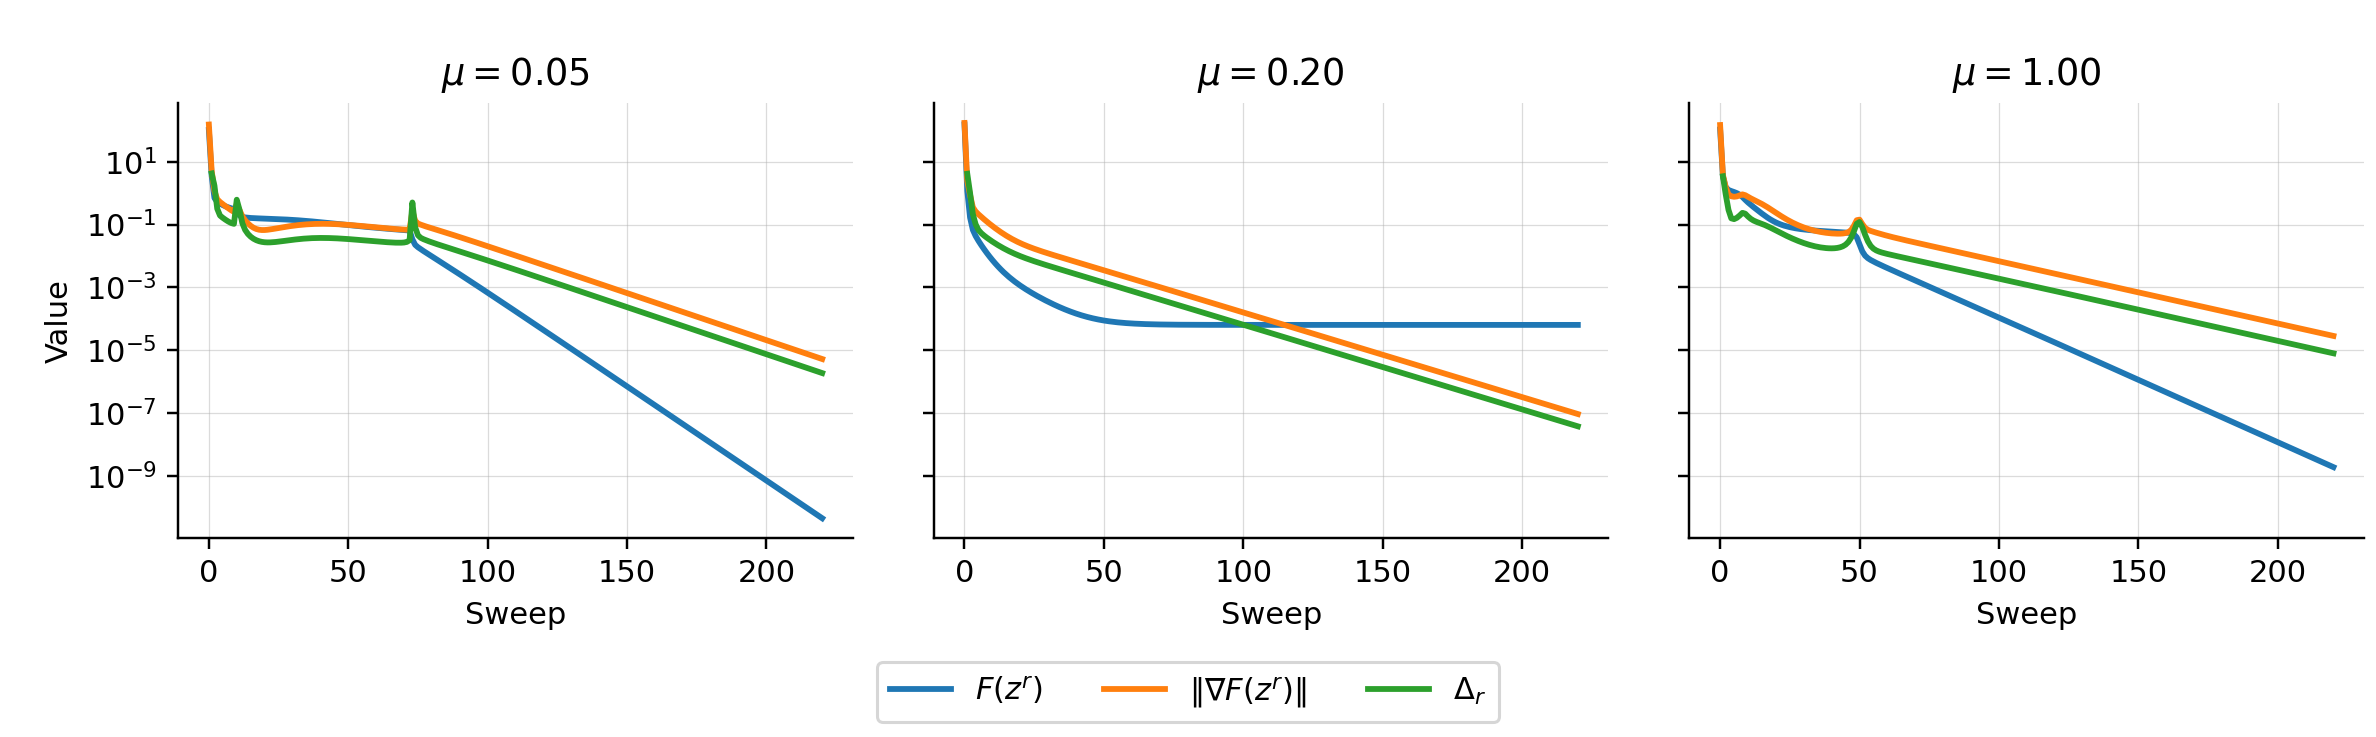
\includegraphics[width=0.95\linewidth]{convergence_history.pdf}
\caption{Convergence histories for low-objective runs with \(\mu=0.05\), \(\mu=0.20\), and \(\mu=1.00\).  Each panel reports the objective value, the free-gradient norm, and the sweep-step size.}
\label{fig:history}
\end{figure}

\begin{figure}[ht]
\centering
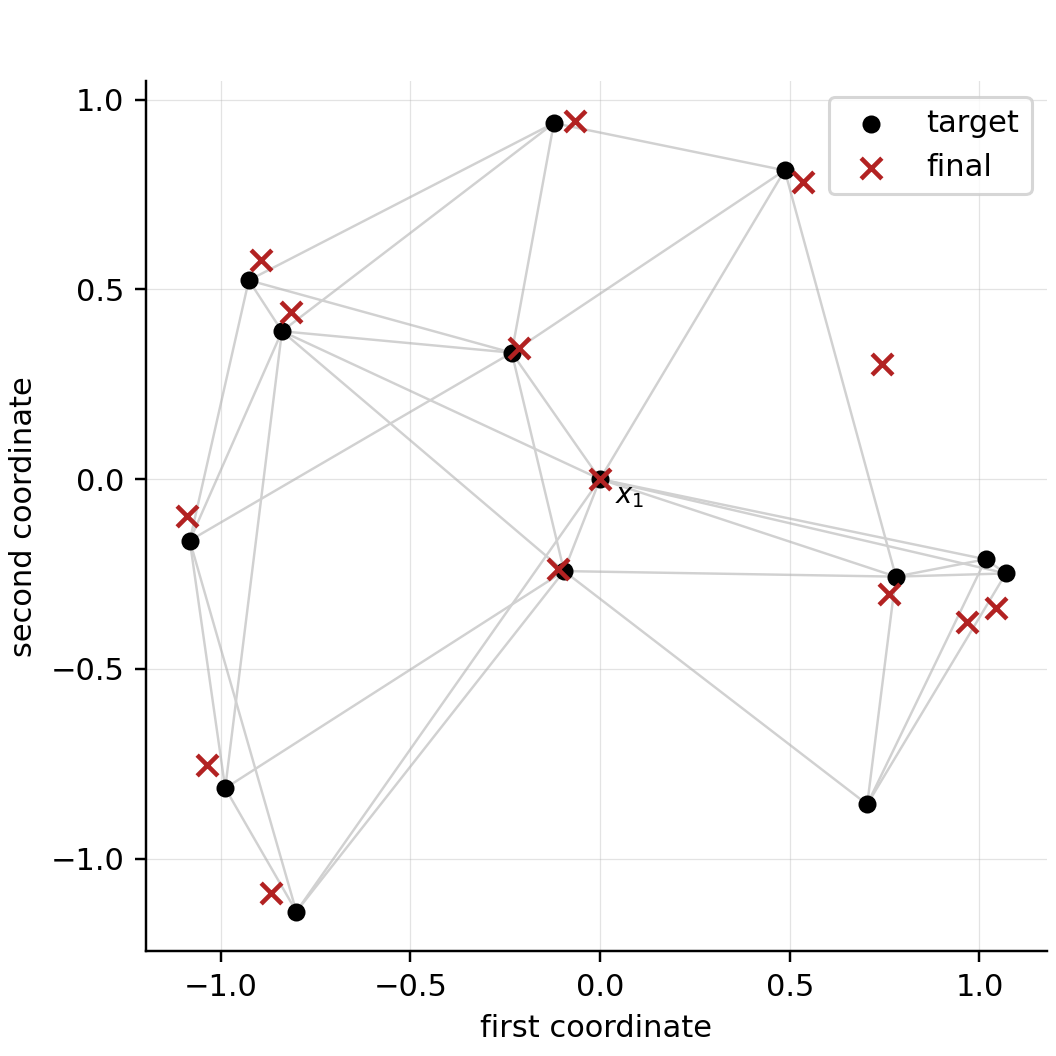
\includegraphics[width=0.82\linewidth]{final_embedding.pdf}
\caption{Planted target realization (circles) and final proximal BCD iterate (crosses) for the low-objective run with \(\mu=0.20\), after optimal orthogonal alignment fixing \(x_1\).}
\label{fig:embedding}
\end{figure}

\clearpage

\section{Conclusion}
\label{sec:conclusion}

The proximal term supplies the missing sufficient-decrease estimate
\[
    F(z^r)-F(z^{r+1})
    \ge
    \frac{\mu}{2}\|z^{r+1}-z^r\|^2,
\]
which rules out the tie-cycle behavior that can occur in exact cyclic block minimization without regularization.  Together with bounded anchored level sets, a relative error estimate, and the polynomial KL property, this yields convergence of the whole proximal cyclic BCD sequence to a stationary point in any fixed Euclidean dimension \(K\ge1\).

\bibliographystyle{plain}
\bibliography{references}

\end{document}
